
\vspace{-0.2cm}
\section{Experiment}\label{sec:exp}
\vspace{-0.2cm}
In this section, we present the experimental results to validate the effectiveness of the proposed BAT algorithm on benchmark datasets and compare it with state-of-the-art baseline methods. We also verify that both two components are helpful and necessary for BAT. The implementation of the BAT can be found via \url{https://anonymous.4open.science/r/benign-adv-77C5}.

\vspace{-0.2cm}
\subsection{Experimental Setup}
\vspace{-0.1cm}
%\jt{we can put baselines here.} \\
%\jt{implementation details, such as optimization method}
In this work, in order to demonstrate the 
merit of BAT, we conduct the experiments mainly on benchmark datasets CIFAR100~\cite{krizhevsky2009learning} and Tiny~ImageNet~\cite{le2015tiny}, which are relatively complex datasets (i.e., containing larger fractions of atypical samples). For both datasets, we study the algorithms under the model architectures ResNet and WideResNet (WRN)~\cite{he2016deep}. In this section, we only present the results of ResNet18 for CIFAR100 and ResNet32 for Tiny~ImageNet and leave the results on WRN in Appendix~\ref{app:exp}. As a fair comparison with BAT, we implement the baseline algorithms including PGD adversarial training~\cite{madry2017towards} as well as its most popular variant TRADES~\cite{zhang2019theoretically}. In addition, we include several recent algorithms: MART~\cite{wang2019improving} and GAIRAT~\cite{zhang2020geometry}, which also incorporate reweighting strategies into adversarial training. For BAT and all baseline methods, we run the algorithms using SGD~\cite{bottou2010large} for 160 epochs with the learning rate that starts from 0.1 and decays by 0.1 after the epoch 80 and 120. More implementation details can be found in Appendix~\ref{app:exp}.

\textbf{Performance on CIFAR100.} For a comprehensive comparison between different methods on CIFAR100, in the results from Table~\ref{Tab:results_cifar100}, we report the models' clean accuracy and adversarial accuracy against $l_\infty$-$8/255$ PGD attack~\cite{madry2017towards}, as well as their performance on the typical sample set and atypical sample set (as described in Section~\ref{sec:pre}). A more comprehensive robustness evaluation on different attacking methods (including CW~\cite{carlini2017towards} and Auto-Attack~\cite{croce2020reliable}) are presented in Appendix~\ref{app:exp}. For BAT, we report its performance when choosing its optimal hyperparameter: $\alpha = 1  ~\text{\&} ~2$ and $\beta = 0.2$. In the Section~\ref{sec:ablation}, we will discuss the impact of the selection of $\alpha$ and $\beta$ on BAT. For baseline methods, the settings and checkpoint selections follow the original papers' suggestions.

%Note that the main goal of BAT is not to improve model's adversarial robustness, so we leave the robustness evaluation with additional attacking methods, such as CW~\cite{carlini2017towards} and Auto Attack~\cite{croce2020reliable} in  Appendix~\ref{app:exp} where we have similar observations.

\vspace{-0.3cm}
\begin{table}[h]
\small
\centering
\caption{Performance of BAT vs. Baselines on CIFAR100 Under ResNet18}
\begin{tabular}{c|cc|cc|cc}
\hline
Method & All Acc. & All Adv. & Typical Acc. & Typical Adv. & Atyp. Acc. & Atyp. Adv. \\
\hline
\hline
PGD Train (Best Adv.) & 56.9 & 27.4 & 90.6 & 59.0 &29.5 & 7.7\\
PGD Train (Best Clean) & 57.8 & 21.9 & 88.3 & 51.0 & \textbf{40.1} & 8.3 \\
%TRADES ($1/\lambda = 1$) & \textbf{61.3} & 21.9 & \textbf{93.0} & 50.0 & 44.7 & 7.9\\
TRADES ($1/\lambda = 5$) & 56.6 & 26.9 & 88.9 & 57.1 & 37.3 & \textbf{10.9} \\
MART~\cite{wang2019improving} & 51.8 & \textbf{30.4} & 85.3 & \textbf{62.2} & 25.3 & 10.1\\
GAIRAT~\cite{zhang2020geometry} & 58.2 & 27.8 & 90.6 & 60.7 & 31.6 & 8.2\\
\hline
BAT ($\alpha = 1, \beta = 0.2$) & \textbf{59.5} &27.3 & \textbf{92.3} & 58.8 & 36.3 & 8.7 \\
BAT ($\alpha = 2, \beta = 0.2$) &59.3 & 27.4 & \textbf{92.3} & 60.3 & 33.1 & 7.4 \\
\hline
\hline
\end{tabular}
\label{Tab:results_cifar100}
\end{table}
\vspace{-0.2cm}
From the results in Table~\ref{Tab:results_cifar100}, we can find that BATs enjoy good clean \& adversarial accuracy trade-off among all methods. It is because BATs can obtain the highest overall clean accuracy ($\sim59.5\%$), as well as comparably good adversarial accuracy ($\sim27.3$) with baseline methods. The only exception is MART~\cite{wang2019improving} which has the higher adversarial accuracy around $\sim 30\%$. However, MART~\cite{wang2019improving} has much lower clean accuracy than BATs. 

To gain a deeper understanding of the working mechanism of BAT, we focus on the performance on BAT vs. PGD adversarial training~\cite{madry2017towards}. Compared with PGD adversarial training with highest adversarial accuracy (PGD Train (Best Adv.)), the BAT methods are $2\sim3\%$ higher in terms of overall clean accuracy, and similar adversarial accuracy. The improvement of clean accuracy is mainly due to BATs' capacity to fit much more atypical samples. For example, the clean accuracy of BAT ($\alpha=1, \beta=0.2$) is about $6\%$ higher than PGD Train~(Best Adv.). On the other hand, compared to PGD adversarial training with the highest clean accuracy (PGD Train (Best Clean)), BATs have much better overall adversarial robustness and slightly better clean accuracy. This is mainly due to BAT's advantage on typical samples, because BATs can successfully prevent the performance drop of typical samples during the training process. Since BATs can achieve good performance on both typical samples and atypical samples, BATs outperform PGD adversarial training in CIFAR100.

\begin{wrapfigure}{r}{0.6\textwidth}
\vspace{-0.4cm}
\subfloat{
\begin{minipage}[c]{0.3\textwidth}
\centering
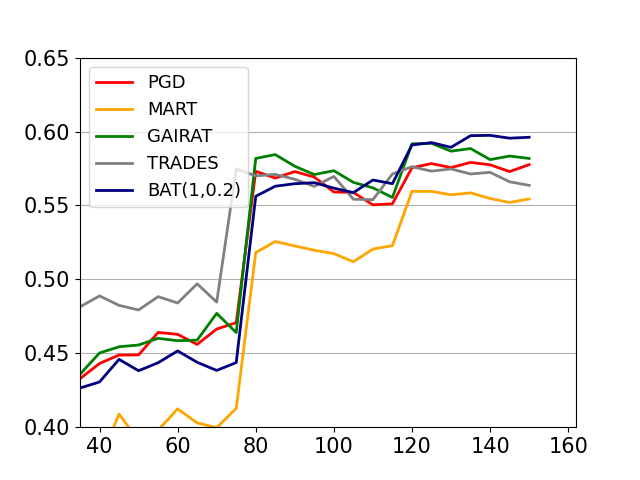
\includegraphics[width = 1.1\textwidth]{figures/base_clean.png}
\end{minipage}
}
\subfloat{
\begin{minipage}[c]{0.3\textwidth}
\centering
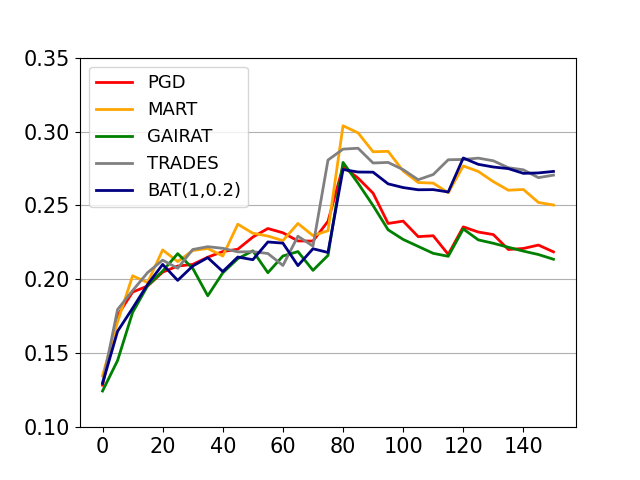
\includegraphics[width = 1.1\textwidth]{figures/base_rob.png}
\end{minipage}
}
\vspace{-0.4cm}
\caption{\small Clean Acc. (left) \& Adv. Acc (right)}
\label{fig:exp1}
\end{wrapfigure}
In Fig.~\ref{fig:exp1}, we also show the change of each models' overall clean accuracy (Fig~\ref{fig:exp1} (left)) \& adversarial accuracy (Fig~\ref{fig:exp1} (right)) along with the training progress. 
Interestingly, similar to PGD adversarial training, all baseline methods cannot achieve the optimal clean and adversarial accuracy at the same moment.
They always achieve the best adversarial accuracy around Epoch 80 (right after the first time weight decay), and the best clean accuracy on the last epochs. However, for BATs, since they can effectively prevent the robustness dropping in the late epochs, BATs are able to train until last epochs and enjoy good clean and adversarial accuracy simultaneously.
%As a result, BATs have higher clean accuracy than all baseline models, and good adversarial accuracy, which are similar or comparable to all baselines (even on their best checkpoints).

\textbf{Performance on Tiny~ImageNet.} Tiny~ImageNet~\cite{le2015tiny} contains 200 classes of the images in the original ImageNet~\cite{krizhevsky2012imagenet} dataset, with 500 training images for each class, and image size $64\times 64$. In our experiments, we only choose the first 50 classes in Tiny ImageNet for training and prediction. Since the image size is $64\times 64$, for both training and robustness evaluation, we consider the adversarial attacks are bounded by $l_\infty$-norm-4/255. In Table~\ref{Tab:results_imagenet}, we report the performance of BAT and baseline methods. Similar to the conclusions we can make from CIFAR100, BATs can achieve the highest overall clean accuracy and comparably good adversarial accuracy with baseline methods. 
\begin{table}[h]
\small
\vspace{-0.2cm}
\centering
\caption{Performance of BAT vs. Baselines on Tiny~ImageNet Under ResNet32}
\begin{tabular}{c|cc|cc|cc}
\hline
Method & All Acc. & All Adv. & Typical Acc. & Typical Adv. & Atyp. Acc. & Atyp. Adv. \\
\hline
\hline
Adv. Train (Best Adv.) & 56.3 & 32.3 & 97.5 & 85.3 &41.5 & 9.6\\
Adv. Train (Best Clean) & 58.2 & 30.5 & 98.0 & 80.4 & 44.7 & 9.1 \\
TRADES ($1/\lambda = 5$) & 55.4 & 28.8 & 97.3 & 77.4 & 38.8 & 9.6 \\
MART~\cite{wang2019improving} & 56.2 & \textbf{34.5} & 97.7 & 85.1 & 41.4 & \textbf{13.6} \\
GAIRAT~\cite{zhang2020geometry} & 58.4 & 30.4 & 98.0 & 81.7 & 45.7 & 7.8\\
\hline
BAT ($\alpha = 1, \beta = 0.2$) & \textbf{59.4} &32.0 & 98.4 & 83.9 & \textbf{48.4} & 10.2 \\
BAT ($\alpha = 2, \beta = 0.2$) &\textbf{59.4} &32.9 & \textbf{99.1} & \textbf{86.9} & 45.7 & 10.9 \\
\hline
\hline
\end{tabular}
\label{Tab:results_imagenet}
\end{table}

\vspace{-0.7cm}
\subsection{Ablation Study}\label{sec:ablation}
\vspace{-0.2cm}
\begin{wrapfigure}{r}{0.6\textwidth}
\vspace{-0.9cm}
\subfloat{
\begin{minipage}[c]{0.32\textwidth}
\centering
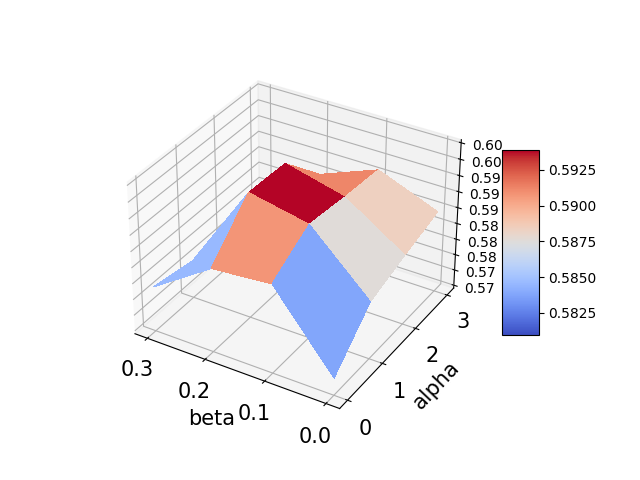
\includegraphics[width = 1.1\textwidth]{figures/abl_clean.png}
\end{minipage}
}
\subfloat{
\begin{minipage}[c]{0.32\textwidth}
\centering
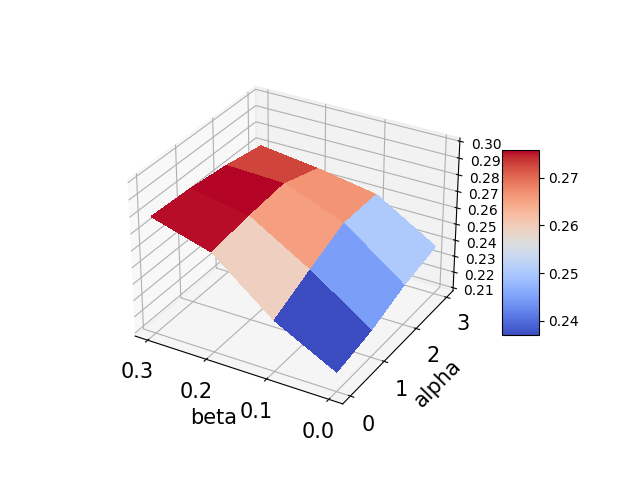
\includegraphics[width = 1.1\textwidth]{figures/abl_rob.png}
\end{minipage}
}
\caption{\small Clean Acc.(left) \& Adv. Acc.(right)}
\label{fig:exp2}
\vspace{-0.2cm}
\end{wrapfigure}
In this subsection, we study the potential impact of the hyperparameters chosen in BAT, which is $\alpha$ that controls the \textit{Reweighting} process and $\beta$ that controls the \textit{Discrimination Loss}. 
In Fig.~\ref{fig:exp2}, we conduct the experiments on CIFAR100 with BAT when $\alpha$ is chosen in [0,1,2,3] and $\beta$ is in [0, 0.1, 0.2, 0.3].
In Fig.~\ref{fig:exp2}, we show each model's overall clean accuracy~(left) \& adversarial accuracy~(right) along the Z-axis, and X-axis / Y-axis indicate the models' corresponding variables of $(\alpha,\beta)$. Note that when $\alpha=\beta=0$, the BAT method regresses to original PGD adversarial training. From the result, we can see that a positive pair of $(\alpha,\beta)$ can benefit both model clean and adversarial accuracy. Therefore, both two components \textit{Reweighting} and \textit{Discrimination Loss} of BAT are helpful and necessary. However, when $\alpha$ or $\beta$ is relatively too large, it will hurt the BAT's clean accuracy. As a result, in CIFAR~100, when $\alpha=1$ or 2 and $\beta= 0.2$, BAT can achieve the optimal performance.

%If we look at the performance of these models at their final epochs, we first observe that $\beta=0.2$ can improve both clean and adversarial accuracy, compared to all models with $\beta = 0$. Moreover, given any fixed value of $\beta$, the model with $\alpha = 1$ or 2 always outperforms than $\alpha=0$.
%Since a positive $\alpha$ indicates the BAT algorithm downweight or exclude certain samples during the training process, we can conclude that those  samples which are downweighted/excluded are acting like poisoning samples to deteriorate the models' performance. and necessary.
